\documentclass[tikz,border=3pt]{standalone}
\usepackage[utf8]{inputenc}
\usepackage[T1]{fontenc}
\usepackage{lmodern}
\renewcommand{\familydefault}{\sfdefault}
\usepackage{sansmath}\sansmath
\usepackage{chemfig}
\usepackage{pgfplots}\pgfplotsset{compat=1.18,/pgf/number format/use comma,/pgf/number format/1000 sep={.}}
\usetikzlibrary{arrows.meta,calc,positioning,decorations.pathmorphing,patterns}
% paleta del sitio
\definecolor{nar}{HTML}{E8680C}\definecolor{narc}{HTML}{FFB35C}\definecolor{hielo}{HTML}{FFF3E8}
\definecolor{tinta}{HTML}{1D1D1F}\definecolor{gris}{HTML}{6E6E73}\definecolor{lila}{HTML}{7C5CF0}
\definecolor{azul}{HTML}{2F6FD6}\definecolor{menta}{HTML}{17A673}\definecolor{coral}{HTML}{E8342A}
\begin{document}
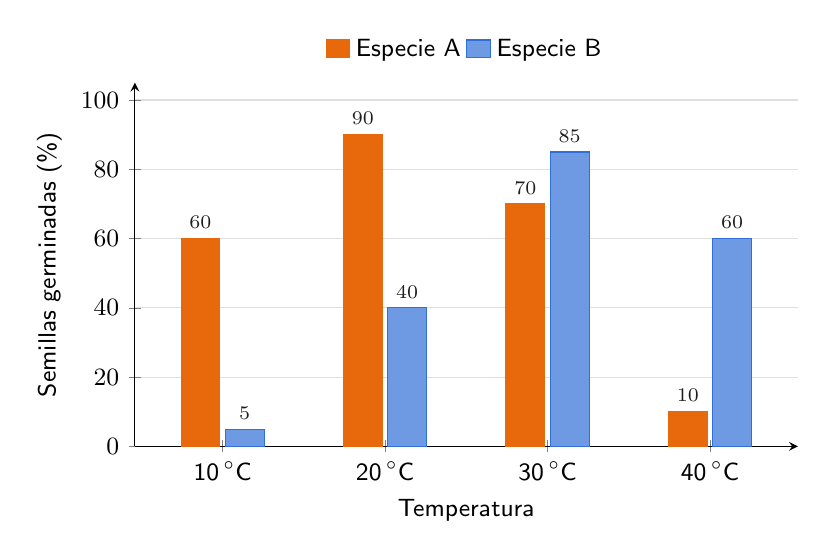
\begin{tikzpicture}[font=\small]
\begin{axis}[width=10cm,height=6.2cm,ybar,bar width=14pt,axis lines=left,ymin=0,ymax=105,ytick={0,20,...,100},
  symbolic x coords={10,20,30,40},xtick=data,xticklabels={10\,$^\circ$C,20\,$^\circ$C,30\,$^\circ$C,40\,$^\circ$C},enlarge x limits=0.18,
  ymajorgrids,grid style={gray!25},xlabel={Temperatura},ylabel={Semillas germinadas (\%)},
  nodes near coords,every node near coord/.append style={font=\scriptsize,text=tinta},
  legend style={at={(0.5,1.03)},anchor=south,legend columns=2,draw=none,font=\small},legend image code/.code={\fill[#1] (0cm,-0.1cm) rectangle (0.3cm,0.12cm);}]
\addplot[fill=nar,draw=nar] coordinates {(10,60)(20,90)(30,70)(40,10)};
\addplot[fill=azul!70,draw=azul] coordinates {(10,5)(20,40)(30,85)(40,60)};
\legend{Especie A\quad,Especie B}
\end{axis}
\end{tikzpicture}
\end{document}
